\documentclass[11pt,a4paper]{article}
\usepackage[T1]{fontenc}
\usepackage[utf8]{inputenc}
\usepackage{amsmath,amsthm}
\usepackage{newtxtext,newtxmath}
\usepackage[scaled=0.94]{sourcesanspro}
\usepackage[margin=23mm,headheight=23pt,headsep=9mm,footskip=12mm]{geometry}
\usepackage{microtype}
\usepackage{xcolor,graphicx,tikz}
\usetikzlibrary{arrows.meta,positioning,calc,decorations.pathmorphing}
\usepackage[most]{tcolorbox}
\usepackage{booktabs,tabularx,array,longtable}
\usepackage{enumitem,fancyhdr,titlesec,caption,float,needspace}
\usepackage{url}
\usepackage[colorlinks=true,linkcolor=Plum,citecolor=Teal,urlcolor=Teal,bookmarksnumbered=true]{hyperref}
\definecolor{Plum}{HTML}{30213F}
\definecolor{Deep}{HTML}{1B1729}
\definecolor{Gold}{HTML}{BF944C}
\definecolor{Glow}{HTML}{EACB87}
\definecolor{Teal}{HTML}{176C80}
\definecolor{Cyan}{HTML}{6ADAE7}
\definecolor{Ink}{HTML}{27303B}
\definecolor{Muted}{HTML}{65717D}
\definecolor{Pale}{HTML}{F5F2EB}
\definecolor{Lilac}{HTML}{F1EDF6}
\definecolor{Rule}{HTML}{DCD6CB}
\hypersetup{pdftitle={Surf the Exponential: From Counterexamples to New Capabilities and Viable Markets},pdfauthor={Vincent Boucher},pdfsubject={Transformational Intelligence and ALPHA GENESIS FLYWHEEL Omega},pdfkeywords={transformational intelligence, constructive challenge, counterexample-guided synthesis, frontier replay, economic invention}}
\ifdefined\pdfinfoomitdate\pdfinfoomitdate=1\fi
\ifdefined\pdftrailerid\pdftrailerid{}\fi
\setlength{\parindent}{0pt}
\setlength{\parskip}{6.3pt plus 1pt minus 1pt}
\setlength{\emergencystretch}{2em}
\linespread{1.05}
\raggedbottom
\renewcommand{\arraystretch}{1.22}
\newcolumntype{Y}{>{\raggedright\arraybackslash}X}
\newcolumntype{L}[1]{>{\raggedright\arraybackslash}p{#1}}
\captionsetup{font=small,labelfont={bf,color=Plum},justification=raggedright,singlelinecheck=false}
\titleformat{\section}{\sffamily\Large\bfseries\color{Plum}}{\thesection}{0.7em}{}
\titleformat{\subsection}{\sffamily\large\bfseries\color{Ink}}{\thesubsection}{0.7em}{}
\titleformat{\subsubsection}{\sffamily\normalsize\bfseries\color{Teal}}{\thesubsubsection}{0.6em}{}
\titlespacing*{\section}{0pt}{17pt}{7pt}
\titlespacing*{\subsection}{0pt}{11pt}{4pt}
\setlist[itemize]{leftmargin=1.3em,itemsep=2pt,topsep=3pt}
\setlist[enumerate]{leftmargin=1.7em,itemsep=3pt,topsep=4pt}
\pagestyle{fancy}\fancyhf{}
\fancyhead[L]{\sffamily\small\color{Muted}SURF THE EXPONENTIAL}
\fancyhead[R]{\sffamily\small\color{Muted}Boucher\enspace|\enspace Research edition 1.0}
\fancyfoot[L]{\sffamily\scriptsize\color{Muted}TRANSFORMATIONAL INTELLIGENCE $\infty$}
\fancyfoot[C]{\sffamily\small\color{Gold}\thepage}
\fancyfoot[R]{\sffamily\scriptsize\color{Muted}ALPHA GENESIS FLYWHEEL $\Omega$}
\renewcommand{\headrulewidth}{0.4pt}
\renewcommand{\headrule}{\hbox to\headwidth{\color{Rule}\leaders\hrule height \headrulewidth\hfill}}
\newtcolorbox{insight}[1][]{enhanced,breakable,colback=Lilac,colframe=Plum,boxrule=0pt,borderline west={2pt}{0pt}{Gold},arc=0pt,left=12pt,right=12pt,top=8pt,bottom=8pt,#1}
\newtcolorbox{scopebox}[1][]{enhanced,breakable,colback=Pale,colframe=Rule,boxrule=.5pt,arc=1mm,left=10pt,right=10pt,top=7pt,bottom=7pt,#1}
\newcommand{\eyebrow}[1]{{\sffamily\small\bfseries\color{Teal}\MakeUppercase{#1}}}
\newcommand{\term}[1]{\textbf{#1}}
\newcommand{\genesis}{ALPHA GENESIS FLYWHEEL $\Omega$}
\newcommand{\ti}{Transformational Intelligence}
\newcommand{\repo}{https://github.com/MontrealAI/AGI-Alpha-Invention-Flywheel-Lab}
\newtheorem{definition}{Definition}[section]
\newtheorem{proposition}[definition]{Proposition}
\newtheorem{theorem}[definition]{Theorem}
\newtheorem{corollary}[definition]{Corollary}
\newcommand{\R}{\mathbb{R}}
\newcommand{\E}{\mathbb{E}}
\newcommand{\ind}{\mathbf{1}}
\begin{document}
\begin{titlepage}
\thispagestyle{empty}

\begin{tikzpicture}[remember picture,overlay]
\fill[Deep] (current page.south west) rectangle (current page.north east);
\fill[Plum] ([yshift=52mm]current page.south west) rectangle ([yshift=-84mm]current page.north east);
\draw[Gold,line width=.7pt] ([xshift=12mm,yshift=12mm]current page.south west) rectangle ([xshift=-12mm,yshift=-12mm]current page.north east);
\coordinate (center) at ([xshift=2mm,yshift=-32mm]current page.center);
% The advancing wave: vector geometry, not a performance chart.
\foreach \i in {0,...,21}{
 \pgfmathsetmacro{\off}{\i*.115}
 \draw[Gold!55!Deep,opacity=.43,line width=.4pt]
  ([xshift=-83mm,yshift=-14mm]center) .. controls ([xshift=-24mm,yshift=-38mm]center) and ([xshift=62mm,yshift=-4mm]center) .. ([xshift=43mm,yshift=30mm+\i*0.45mm]center)
  .. controls ([xshift=30mm,yshift=54mm+\i*.35mm]center) and ([xshift=-12mm,yshift=30mm]center) .. ([xshift=9mm,yshift=12mm+\i*.5mm]center);
}
\draw[Cyan,line width=1.5pt] ([xshift=-83mm,yshift=-14mm]center) .. controls ([xshift=-24mm,yshift=-38mm]center) and ([xshift=62mm,yshift=-4mm]center) .. ([xshift=43mm,yshift=34mm]center) .. controls ([xshift=30mm,yshift=57mm]center) and ([xshift=-12mm,yshift=30mm]center) .. ([xshift=9mm,yshift=18mm]center);
\node[text=Glow,font=\fontsize{48}{50}\selectfont] at ([xshift=12mm,yshift=1mm]center) {$\infty$};
\fill[Cyan] ([xshift=9mm,yshift=18mm]center) circle (1.2mm);
\node[text=Glow,font=\sffamily\small,anchor=west] at ([xshift=22mm,yshift=-22mm]current page.north west) {MONTREAL.AI\enspace /\enspace QUEBEC.AI};
\node[text=Glow,font=\sffamily\small,anchor=east] at ([xshift=-22mm,yshift=-22mm]current page.north east) {RESEARCH EDITION 1.0};
\node[text=white,font=\sffamily\bfseries\fontsize{49}{52}\selectfont,anchor=west] at ([xshift=22mm,yshift=-53mm]current page.north west) {SURF THE};
\node[text=Glow,font=\sffamily\bfseries\fontsize{37}{43}\selectfont,anchor=west] at ([xshift=22mm,yshift=-72mm]current page.north west) {EXPONENTIAL};
\node[text=white,align=left,anchor=north west,text width=158mm,font=\large] at ([xshift=23mm,yshift=-86mm]current page.north west) {From Counterexamples to New Capabilities,\\Viable Markets, and Better Discovery};
\node[text=Glow,font=\sffamily\bfseries\large,anchor=west] at ([xshift=23mm,yshift=72mm]current page.south west) {ALPHA GENESIS FLYWHEEL $\Omega$};
\node[text=white,align=left,anchor=west,font=\large] at ([xshift=23mm,yshift=57mm]current page.south west) {Challenge the claim. Change the game.\\Build what becomes possible.};
\node[text=white,align=left,anchor=south west,font=\normalsize] at ([xshift=23mm,yshift=24mm]current page.south west) {\textbf{Vincent Boucher}\\Montr\'eal, Qu\'ebec, Canada};
\node[text=Glow,align=right,anchor=south east,font=\sffamily\small] at ([xshift=-23mm,yshift=24mm]current page.south east) {TRANSFORMATIONAL INTELLIGENCE $\infty$\\5 November 2026};
\end{tikzpicture}
\null
\end{titlepage}
\setcounter{page}{1}
\eyebrow{A constructive theory of challenge}
\begin{center}
{\sffamily\LARGE\bfseries\color{Plum}SURF THE EXPONENTIAL}\par
\vspace{4pt}
{\Large From Counterexamples to New Capabilities,\\Viable Markets, and Better Discovery}\par
\vspace{8pt}
Vincent Boucher\quad$\cdot$\quad MONTREAL.AI / QUEBEC.AI\par
{\small Montr\'eal, Qu\'ebec, Canada\quad$\cdot$\quad 5 November 2026}
\end{center}
\eyebrow{Abstract}
A fluent summary can omit the chapter that changes its meaning. A second language model may expose the omission, but only if it can inspect the relevant source and its criticism is itself checked. We develop this intuition into \emph{constructive challenge}: use an adjudicated counterexample not only to reject a claim, but to identify and construct the missing means of achieving the original purpose. Building on \ti, \genesis, and \emph{Invent the Economy}, the proposal connects source-grounded criticism, reformulation, capability construction, voluntary exchange, and tested successor benefit. It challenges both premature success and premature impossibility, while keeping user purpose, evaluation, and execution authority separate. We derive a source-information limit, a conditional critic-dependence calculation, and a standard flow-based composition criterion that turns a failed portfolio promise into a concrete construction requirement. A new executable finite study detects two individually feasible promises that overbook one resource. After an authored capability-cost change, a technical adapter and a pooled reservation arrangement jointly reduce complete modeled cost from 17 to 13 units against 16 units of conditional receipts; either change alone remains insufficient. An independently implemented conventional oracle matches the constructor across all 192 declared parameter cases: 63 admissions and 129 refusals. Thirty-eight tests pass in normal and optimized Python. These are exact supplied-model results, not frontier-model performance, actual contracts, customer receipts, or achieved self-improvement. The research objective is an enterprise that converts a verified objection into a better construction---and converts that construction into a demonstrably useful advantage for discovering what comes next.

\begin{scopebox}
\textbf{What is new here.} A synthesis and operating contract for turning material criticism into constructive opportunity search; a runnable composition-and-economics laboratory; explicit tests of misleading acceptance, unnecessary invention, and ordinary-method ties; and a falsifiable programme for evaluating the complete discovery loop. No second LLM, customer transaction, or external institutional audit was executed in the companion.
\end{scopebox}
{\small\textbf{Keywords:} transformational intelligence; constructive challenge; counterexamples; frontier replay; economic possibility; capability inheritance; cyber resilience.}
\newpage
\eyebrow{The paper in one minute}
\section*{Do not merely find the flaw.\\Build the possibility it reveals.}
A reader asks an AI to summarize a book. The summary sounds excellent. A challenger opens the book and discovers that the conclusion depends on a condition the summary omitted. The first gain is a better answer. The deeper gain is a better way of producing answers: preserve the important claims and their dependencies before compressing them.

Now replace the book with a business promise. Two customers each receive a valid-looking backup-fulfillment plan. A challenger combines them and finds that both plans rely on the same four units of capacity. Eight units have been promised. Four exist. More confident prose cannot deliver the missing four.

The objection can become an invention target. Can a different production interface make an otherwise incompatible supplier usable? Can an accepted reservation arrangement make that supplier affordable? Can we construct the two changes together, test the complete portfolio, and preserve the customer outcome?

\begin{insight}
\textbf{The creative move is not a more persuasive defense of the original plan. It is a better arrangement for making the original promise true.}
\end{insight}

\begin{figure}[H]\centering
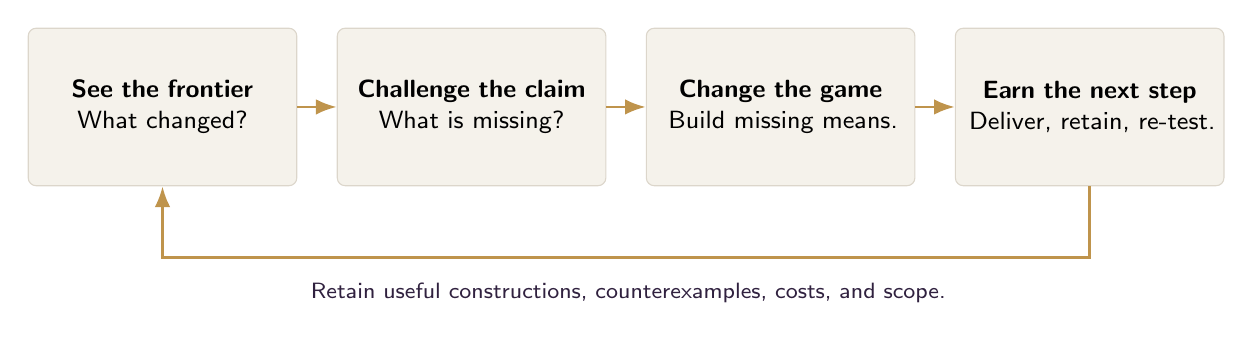
\begin{tikzpicture}[node distance=5mm,font=\sffamily\small,>=Latex]
\tikzset{box/.style={draw=Rule,fill=Pale,rounded corners=1mm,text width=32mm,inner sep=3pt,minimum height=20mm,align=center},arrow/.style={->,line width=1pt,draw=Gold}}
\node[box] (a) {\textbf{See the frontier}\\What changed?};
\node[box,right=of a] (b) {\textbf{Challenge the claim}\\What is missing?};
\node[box,right=of b] (c) {\textbf{Change the game}\\Build missing means.};
\node[box,right=of c] (d) {\textbf{Earn the next step}\\Deliver, retain, re-test.};
\draw[arrow](a)--(b);\draw[arrow](b)--(c);\draw[arrow](c)--(d);
\draw[arrow](d.south)--++(0,-9mm)-|(a.south);
\node[below=11mm of $(b.south)!.5!(c.south)$,text=Plum,text width=145mm,align=center,font=\sffamily\footnotesize] {Retain useful constructions, counterexamples, costs, and scope.};
\end{tikzpicture}
\caption{The proposed constructive loop. Arrows are obligations to demonstrate a connection, not declarations that the connection has already been achieved.}
\end{figure}

\textbf{Three questions govern the enterprise.} What can we now do? What valuable activity does that make possible? What would improve our ability to discover and realize the next activity? Criticism serves all three: it can expose an unavailable capability, a missing economic condition, or a mistaken discovery method.

\textbf{Read by purpose.} Sections 1--4 explain the mechanism. Sections 5--7 formalize and execute it. Sections 8--10 connect it to actual commerce and successor learning. Sections 11--13 specify evaluation, boundaries, and the research horizon. Appendices provide proofs, reproduction, and the paper's own adversarial review.
\newpage
\setcounter{tocdepth}{1}
\tableofcontents
\newpage
\section{The missing chapter can become the next invention}
The useful asymmetry in the opening example is between producing a convincing artifact and exposing a specific consequential defect. A reader may not know how to assess an entire book summary, yet may be able to inspect a cited passage and determine that a central qualification was lost. Debate, tool-grounded critique, and prover--verifier research provide important precedents for making difficult outputs more checkable \cite{irving,gou,kirchner}. They do not imply that a second model is automatically right.

The motivating example is already developed in \emph{Transformational Intelligence: Learning to Change the Game}, including the possibility of replacing a summarize-then-criticize workflow with source-grounded construction \cite[Sec.~1; App.~C]{ti}. This paper takes that starting point further in a specific direction: \term{an upheld objection can identify a missing productive means}. A missing chapter can suggest a dependency-preserving representation; an overbooked supplier can suggest a portfolio reservation mechanism; an unfinanceable delivery can suggest a different construction or payment sequence. The transformation is useful only when the replacement works for the authorized purpose.

\subsection{From criticism as a filter to criticism as a construction input}
A filter answers whether a candidate should be admitted. A constructive challenge additionally asks what must change for a worthwhile outcome to become achievable. It does not require every rejected idea to be rescued. Sometimes the evidence supports the incumbent, a smaller authorized scope, a different opportunity, or stopping. The point is to make rejection informative enough to guide a legitimate next decision.

We distinguish three outputs. A \emph{defect witness} establishes a particular failure of a claim. An \emph{obstruction hypothesis} explains why the failure recurs. A \emph{construction proposal} identifies a new representation, observation, process, interface, or arrangement that might remove it. The witness can be established while the explanation remains uncertain and the construction unbuilt. Collapsing the three into one confident criticism recreates the original problem.

For example, a double booking establishes incompatible assignments under a specified shared-capacity model. It does not prove that the business is impossible, that all capacity markets fail, or that a blockchain is required. The next investigation might discover another supplier, a cheaper compatible interface, a genuinely feasible joint schedule, or that the promised price cannot cover a competent delivery route. Each has a different evidential burden.

\subsection{The positive objective survives the challenge}
A system rewarded for finding objections can produce an endless objection machine. A system rewarded for defending proposals can produce an endless persuasion machine. Neither is the desired enterprise. The outcome remains worthwhile construction and delivery, not the number of criticisms, the length of debate, or a judge's confidence.

\begin{insight}
\textbf{Challenge success claims and impossibility claims.} A valid counterexample can show that a proposed solution fails. A valid construction can show that a claim of impossibility was too broad. Both directions belong in the same discovery process.
\end{insight}

\section{Three foundations, one additional operating link}
This manuscript preserves the three supplied papers' distinct objects of invention. It does not treat them as reports of capabilities they explicitly leave unestablished.

\begin{table}[H]\small
\begin{tabularx}{\textwidth}{@{}L{37mm}YY@{}}\toprule
\textbf{Foundation} & \textbf{What it makes editable} & \textbf{What this paper adds}\\\midrule
\ti\ \cite{ti} & The problem-solving formulation, while preserving purpose and separately validating changes to evaluation. & A criticism-to-construction record that identifies the violated obligation and a testable alternative means.\\
\genesis\ \cite{genesis} & Frontier interpretation, consequence discovery, and the machinery that discovers useful capabilities. & Replay driven by specific unresolved obstructions; comparison of the institution's contribution with better models and ordinary tools.\\
\emph{Invent the Economy}\ \cite{economy} & The capability and voluntary commercial arrangement, including financing, rights, and delivery timing. & Challenges to composed promises, reservation capacity, unsupported consent, and the complete route from accepted result to successor.\\\bottomrule
\end{tabularx}
\caption{Source-derived foundations and the additional synthesis. The source papers' earlier exact studies and operating simulations are not re-executed or upgraded by this publication.}
\end{table}

\ti\ separates the intent charter, formulation, and evaluation instrument \cite[Secs.~2, 7]{ti}. GENESIS separates seeing the frontier, seeing its consequences, and improving discovery; it adopts a capable existing route when that route wins \cite[Secs.~3, 12]{genesis}. \emph{Invent the Economy} separates technical possibility, modeled viability, accepted arrangement, realized exchange, and repeatable market \cite[Sec.~2.2]{economy}. These separations are retained throughout.

Our additional link is \term{adjudicated criticism $\rightarrow$ missing-means construction $\rightarrow$ purpose-grounded acceptance $\rightarrow$ tested reuse}. The extended object includes the criticized claim, its source, the actual obstruction, a proposed change, the decisive experiment, an allowed realization, and the evidence needed for any stronger next claim.

\subsection{What is not claimed as new}
Counterexample-guided inductive synthesis (CEGIS) already alternates candidate generation with counterexample-producing validation \cite{solar}. Network flow already supplies compositional feasibility tests \cite{ford}. Transformational creativity has a substantial history \cite{boden}. New executable methods and agent improvements already have strong precedents, including AlphaEvolve and GEPA \cite{alphaevolve,gepa}. The present contribution is a purpose-grounded synthesis connecting those mechanisms to frontier adaptation, whole commercial arrangements, and successor attribution, together with a small executable laboratory that can falsify its local claims.

\section{What a trustworthy challenge must contain}
\subsection{Anchor the claim before choosing the critic}
Let an authorized mission be $\mathcal I=(O,H,A,B)$, with intended outcomes $O$, non-negotiable requirements $H$, permissions $A$, and declared resources $B$. Let $F$ describe one formulation and $E$ its evaluation instrument. The paper's claim packet is
\begin{equation}
\mathcal C=(\mathcal I,F,E,x,y,\mathcal S,\Gamma),
\end{equation}
where $x$ is the relevant input, $y$ the candidate artifact or action record, $\mathcal S$ the inspectable source set, and $\Gamma$ the stated scope and evidence status. This notation is an implementation contract, not an assumption that all human purposes are fully formalizable.

A useful obligation graph links purpose requirements to source facts, construction dependencies, acceptance checks, and accountable counterparties. Obligations can be declared requirements, independently established facts, estimates, or unknowns. A missing edge is not automatically a defect: some omitted book details are irrelevant to a summary's purpose. Conversely, a persuasive edge label is not evidence that its prerequisite exists.

\begin{definition}[Material challenge]
A material challenge identifies a stated claim, an authorized requirement or necessary premise, source-bound evidence or an executable counterexample, the consequence for the outcome, and a proposed method for adjudicating the disagreement. It does not itself grant execution authority or establish its own correctness.
\end{definition}

A challenge record should distinguish \emph{refuted}, \emph{supported within scope}, \emph{unresolved}, and \emph{out of scope}. It should state whether the repair is to an answer, a formulation, an evaluator, or an unsupported success label. The adjudicator may reject a criticism. A nonexistent quotation, a harmless omission, or an unpermitted change to the objective is not a productive objection.

\subsection{Four functions, not a mandatory four-agent organization}
The \term{builder} produces the artifact and its claimed bridge to the purpose. The \term{challenger} searches for the most consequential justified counterexample, including a stronger complete alternative. The \term{adjudicator} checks the disputed claim against sources, tests, measurements, or actual counterparties. The \term{constructor} uses an upheld objection to propose and build a better means. One tool can serve multiple functions; separate model instances can still share the same blind spot.

Procedural separation and evidence separation should be explicit. Different prompts do not establish independent training data, independent observations, independent institutions, or statistically independent errors. The companion uses separately coded computations under common authorship. It does not call a second frontier model. This narrower claim is stronger than an unsupported assertion of independent AI certification.

\subsection{Give the critic the equivalent of the book}
For a book, that means the correct edition, the requested length and purpose, source locations, and the summary. For recovery, it means the authorized business obligations, source records, recovery assumptions, and current fulfillment status. For commerce, it also means accepted terms, actual receipts, incurred costs, protected obligations, and supplier commitments. A critic supplied only with the builder's success report can at most examine that report's internal consistency.

Tool-grounded feedback is an important distinction in CRITIC \cite{gou}. Historical self-correction studies also show why improvement should not be assumed from asking for another pass without external feedback \cite{huang}. Those findings motivate access to appropriate evidence; they do not establish the error rates of contemporary models or this proposed enterprise.

\section{Go beyond debate: challenge the setup that produced the error}
\subsection{Three levels of response}
The first response is \term{repair}: restore the omitted qualification or correct the assignment. The second is \term{reformulation}: change how the artifact is produced so the same failure becomes easier to prevent or detect. The third is \term{possibility construction}: use the new means to enable a useful activity that the former setup could not adequately support.

In the book example, repair adds the missing condition. Reformulation constructs a source-linked claim structure before compression. A further possibility, when the user authorizes an understanding task rather than a fixed summary, is an adaptive, evidence-backed instrument for answering the reader's questions. Each change must be evaluated against the actual purpose, not declared better because it is more elaborate \cite[App.~C]{ti}.

In continuity, repair refuses the overbooked promise. Reformulation uses portfolio-level commitments rather than separate views of capacity. A further possibility is a rehearsed arrangement in which qualified providers can fulfill specified obligations during disruption. That arrangement is not created by a feasibility calculation: counterparties must accept it and its resources must be usable.

\subsection{Five legitimate construction moves}
An upheld witness can motivate a better \emph{representation}, a new \emph{observation}, a changed \emph{production interface}, a different \emph{coordination or financing arrangement}, or a better \emph{measurement instrument}. These are hypothesis families, not a universal grammar. A generator must remain able to propose other operations; otherwise the catalogue becomes another restrictive formulation.

A change to evaluation is especially sensitive. The candidate may show that the current judge rewards the wrong output property. The replacement judge then needs separate evidence that it measures the authorized outcome more faithfully; both candidate and incumbent are compared on the common supported basis. The candidate cannot privately change its judge and immediately claim victory \cite[Sec.~7]{ti}.

\subsection{A constructive critic should ask two opposing questions}
First: \emph{What is the strongest supported reason this candidate fails the original objective?} Second: \emph{What is the strongest feasible construction that would defeat our claim that the objective cannot be reached?} The second prevents failure analysis from hardening into a permanent boundary on imagination.

A failed supplier allocation may have a feasible alternative. A rejected research instrument may become practical after a measured capability change. A lower-cost incumbent may make an internal construction unnecessary. A search failure may reflect a weak search procedure rather than a physical limit. The institution should retain the obstruction and its falsifiers, not merely a permanent red label.

\begin{insight}
\textbf{A counterexample is a question addressed to construction: what would have to become true, and what could we actually build to make it true?}
\end{insight}

\section{Formal limits and constructive witnesses}
\subsection{A critic cannot reconstruct information it never receives}
Let $S$ be a source, $T(S)$ the representation shown to a critic, and $g(S,y)$ the correctness of candidate $y$ under the original task.
\begin{proposition}[Indistinguishable-source limit]\label{prop:source}
If $T(S_0)=T(S_1)$ but $g(S_0,y)\ne g(S_1,y)$, no deterministic critic observing only $(T(S),y)$ is correct in both worlds. Under an equal prior over the two worlds, any randomized critic whose randomness is independent of the source has classification accuracy at most $1/2$.
\end{proposition}
\begin{proof}
The critic receives the same input distribution in both worlds and therefore has the same output distribution. The two correct labels are opposite; their equal-weight accuracy sums to $1/2$. An abstention can avoid an unsupported claim but cannot establish which world holds.
\end{proof}
This is an elementary information argument, closely aligned with the source manuscript's observational-ceiling example \cite[Sec.~3]{ti}. It does not prove that real book-summary evaluation is generally impossible. It identifies when inspecting the original source, acquiring a distinguishing observation, or changing the representation is necessary for a stronger claim. Adding more critics to the same insufficient transcript does not fix the missing information.

\subsection{More critics are not automatically more independent evidence}
Let $W$ denote an invalid proposal, $p=\Pr(W)$, and $M_i$ the event that critic $i$ misses it. Then
\begin{equation}
\Pr(W\cap M_1\cap\cdots\cap M_k)=p\prod_{i=1}^{k}\Pr(M_i\mid W,M_1,\ldots,M_{i-1}).\label{eq:critics}
\end{equation}
This is the probability chain rule, not an error guarantee. Replacing the conditional factors with a common marginal miss rate $q$ requires justified conditional independence. In the companion's authored illustration, $p=1/5$, $q=1/4$, and three independent critics leave invalid-and-undetected probability $1/320$. Perfectly correlated misses leave $1/20$. Neither number is a measured LLM property. False objections and adjudication errors require separate accounting.

\subsection{Individual feasibility does not imply portfolio feasibility}
Let $x$ represent commitments made before a disruption. For scenario $\omega$, let $y(\omega)$ allocate surviving usable resources to obligations. A portfolio promise requires
\begin{equation}
\exists x\in X\quad\forall\omega\in\mathcal U\quad\exists y(\omega):\quad G(x,y(\omega),\omega)=\mathrm{true}.\label{eq:robust}
\end{equation}
The same $x$ must work across the declared scenario set. Choosing new reserved capacity after learning the disruption solves a different problem. Our finite experiment assumes the active clients and supplier failure are observed before dispatch. If they are not, recourse policies must additionally agree on observationally indistinguishable histories; Equation~\eqref{eq:robust} alone is then too permissive.

For a single declared activation window, let clients have divisible demands $d_i\ge0$, suppliers usable reserved capacities $c_j\ge0$, and $N(S)$ the suppliers qualified to serve at least one client in subset $S$.
\begin{theorem}[A composition criterion and obstruction witness]\label{thm:cut}
Under the stated divisible-demand, shared-capacity bipartite model, all client demands can be served if and only if
\begin{equation}
\sum_{i\in S}d_i\le\sum_{j\in N(S)}c_j\qquad\text{for every client subset }S.\label{eq:cut}
\end{equation}
A violating subset yields deficit $\delta(S)=\sum_{i\in S}d_i-\sum_{j\in N(S)}c_j>0$. Any successful repair must remove that deficit by changing the eligible usable capacity, the compatibility structure, or an explicitly authorized requirement.
\end{theorem}
\begin{proof}
Necessity follows because only suppliers in $N(S)$ can serve $S$. For sufficiency, construct a source--client--supplier--sink network with source edges $d_i$, supplier--sink edges $c_j$, and sufficiently large compatible client--supplier edges. The subset inequalities make every separating cut at least total demand; max-flow/min-cut gives a saturating flow \cite{ford}. With integer capacities, an integer unit flow exists. A fixed unchanged violating cut remains infeasible, so a valid repair must change one of its relevant terms or edges.
\end{proof}
This is a standard network result used as a constructive interface, not a new flow theorem. It does not cover indivisible jobs, travel times, stochastic quality, hidden capacity commitments, or interacting material constraints without extensions. A computational witness proves the modeled shortage; it does not manufacture a willing supplier.

\subsection{From a cut to a construction specification}
Two clients each need four units. Their independent plans both use supplier $P$, which has capacity four. Both singleton inequalities pass. The combined subset has demand eight and capacity four: $\delta=4$. A constructive search can add four qualified units, make an inaccessible supplier compatible, change the schedule where the purpose permits, or find an existing complete alternative. Merely producing a second signed-looking plan does not change the inequality.

This is the operational bridge from criticism to invention. The objection names the constraint that the next construction must actually change. It avoids both a vague instruction to ``be creative'' and the false conclusion that correcting the prose corrects the world.

\section{SURF: a frontier-adaptive constructive loop}
The title is a strategy, not a fitted exponential law. GENESIS's three functions remain: see a real capability change, see its consequences, and improve the process that constructs those consequences \cite[Secs.~3, 7]{genesis}. Constructive challenge is the link that keeps these functions responsive to evidence rather than attached to their previous story.

\begin{figure}[H]\centering
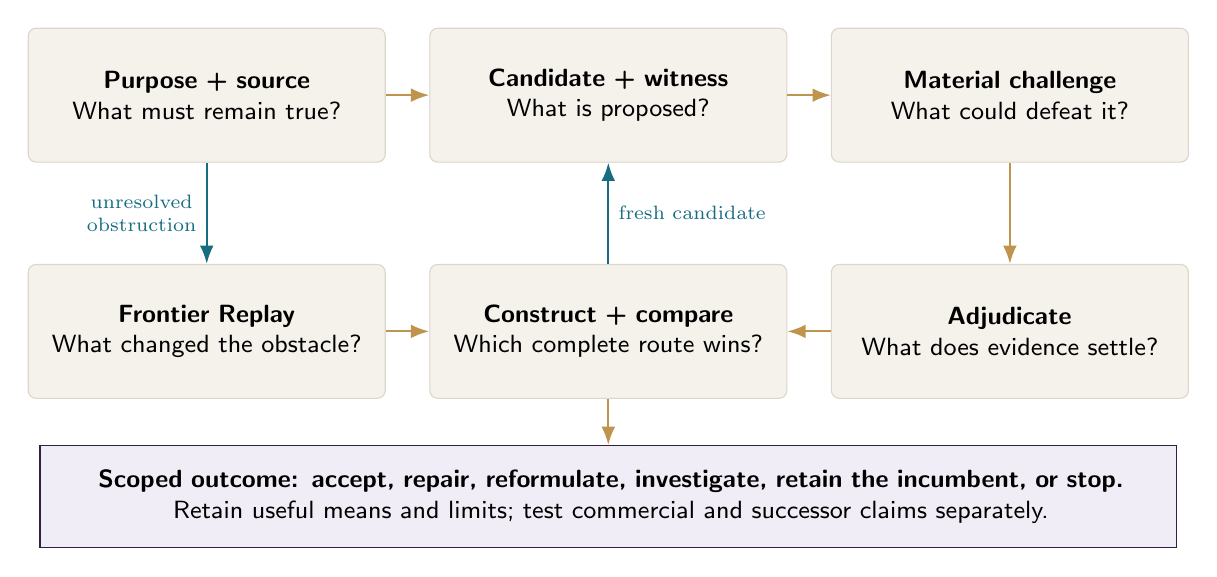
\begin{tikzpicture}[font=\sffamily\small,>=Latex]
\tikzset{n/.style={draw=Rule,fill=Pale,rounded corners=1mm,text width=43mm,minimum height=17mm,align=center}}
\node[n] (source) at (0,0) {\textbf{Purpose + source}\\What must remain true?};
\node[n] (claim) at (5.1,0) {\textbf{Candidate + witness}\\What is proposed?};
\node[n] (challenge) at (10.2,0) {\textbf{Material challenge}\\What could defeat it?};
\node[n] (replay) at (0,-3.0) {\textbf{Frontier Replay}\\What changed the obstacle?};
\node[n] (build) at (5.1,-3.0) {\textbf{Construct + compare}\\Which complete route wins?};
\node[n] (judge) at (10.2,-3.0) {\textbf{Adjudicate}\\What does evidence settle?};
\draw[->,Gold,thick](source)--(claim);\draw[->,Gold,thick](claim)--(challenge);
\draw[->,Gold,thick](challenge)--(judge);\draw[->,Gold,thick](judge)--(build);\draw[->,Gold,thick](replay)--(build);
\draw[->,Teal,thick](build.north)--node[right,font=\scriptsize]{fresh candidate}(claim.south);
\draw[->,Teal,thick](source.south)--node[left,font=\scriptsize,align=center]{unresolved\\obstruction}(replay.north);
\node[draw=Plum,fill=Lilac,text width=142mm,align=center,minimum height=13mm] (outcome) at (5.1,-5.1) {\textbf{Scoped outcome: accept, repair, reformulate, investigate, retain the incumbent, or stop.}\\Retain useful means and limits; test commercial and successor claims separately.};
\draw[->,Gold,thick](build)--(outcome);
\end{tikzpicture}
\caption{A proposed operating architecture. The adjudicator can reject the criticism; a new frontier event can also invalidate the opportunity. Permission and outcome boundaries constrain every route.}
\end{figure}

\subsection{An implementable episode}
\begin{enumerate}
\item \textbf{Bind the purpose and evidence.} Record the claim, task boundary, source identities, known gaps, resources, and permitted actions. Identify which material conditions require external evidence.
\item \textbf{Construct competing complete routes.} Include direct use of the strongest accessible tool, an existing specialist, a proposed construction, and non-entry. Allow new operations to be proposed rather than treating the current catalogue as reality's boundary.
\item \textbf{Challenge in both directions.} Search for a material counterexample to the leading route and a feasible alternative to any broad impossibility claim. Prefer disputes that could change the decision.
\item \textbf{Adjudicate before promotion.} Reproduce the test or inspect the source. Mark unresolved disagreements explicitly. Test the critic's factual basis and relevance; do not reward accusation count.
\item \textbf{Construct the missing means.} Use the upheld obstruction to compare observations, interfaces, production changes, arrangements, and combinations. Count failed attempts and checker construction.
\item \textbf{Freeze and test.} Evaluate the finalist on appropriate fresh work with a capable unrestricted alternative, matched permissions, and complete costs. Revisiting exposed development examples is not fresh confirmation.
\item \textbf{Deliver and retain within scope.} Obtain the relevant external acceptance, reconcile actual collections and obligations where commerce occurs, and preserve reusable artifacts with applicability and invalidation conditions.
\item \textbf{Test the successor.} Ask whether retained means or earned resources improve a different useful activity. Test a changed discovery policy separately from better initial tools or a stronger foundation model.
\end{enumerate}

\subsection{Allocate criticism by decision value}
A reasonable investigation target is an observation whose expected effect on the next allowed decision exceeds its complete acquisition, interpretation, delay, and opportunity costs. In a declared one-step model,
\begin{equation}
\operatorname{VOI}(e)=\E_Z\!\left[\max_{a\in\mathcal A(Z)}\E[J(a)\mid Z,e]\right]-\max_{a\in\mathcal A_0}\E[J(a)]-K_e.\label{eq:voi}
\end{equation}
This uses the source GENESIS decision principle \cite[Sec.~6.2]{genesis}. If the experiment also constructs a reusable instrument, its effect belongs in the continuation state rather than being counted twice as an extra reward. Estimates are uncertain and cannot grant authority. Sometimes the best next action is a small measurement, a direct conventional solution, or stopping rather than more debate.

\section{Executed laboratory: omission, composition, and a newly viable construction}
\subsection{Protocol, scope, and comparators}
The new companion uses Python's standard library, exact integer costs, integer network flow, and a separately coded subset-capacity oracle. Inputs, supplier menus, candidate operations, buyer prices, and scenario sets are authored. There are no model calls, learned probabilities, real buyers, supplier negotiations, field systems, or financial accounts. These are post-design exact-model checks, not a preregistered natural-workload benchmark.

The constructor alternates least-cost selection on the currently exposed scenario constraints with a verifier that searches the complete declared scenario set. The strong conventional oracle instead enumerates the full finite construction set and all subset-capacity inequalities upfront. It reconstructs pricing independently and never calls the producer's flow function. Both have the same permitted constructions and full eventual scenario access. The comparison tests implementation and constraint handling, not an alleged new optimization algorithm.

\subsection{Study A: a critic can inherit an omission}
The authored source contains four required obligations $Q=\{q_1,q_2,q_3,q_4\}$, plus an incidental item not required by the charter. The supplied summary and output omit $q_3$. Comparing the output only with that summary accepts it; source-bound checking rejects it and identifies $q_3$. A legitimate compression omitting only the incidental item passes. Fabricated-source and immaterial criticisms are rejected or classified as irrelevant.

This is a finite obligation-coverage test, not a measurement of book comprehension or the ability of an LLM to discover which passages matter. It demonstrates a verification dependency: an outcome can agree perfectly with a lossy input and still violate the actual requirement. Natural-book experiments must establish materiality separately.

\subsection{Study B: two valid local plans, one impossible joint promise}
Clients $A$ and $B$ each need four interchangeable units in the same window. Supplier $P$ has four usable units. Each singleton plan passes. Their joint demand is eight, and the maximum delivered flow is four. The omitted combined scenario yields the cut witness in Theorem~\ref{thm:cut}.

The constructor initially proposes $P$ alone. Its nominal modeled cost is eight: four reserved-capacity units of cost and four units of fixed and delivery allowance. The complete verifier supplies the simultaneous-activation counterexample. The constructor must now find a genuinely feasible portfolio or decline. It cannot repair the claim by hiding either client.

\subsection{Study C: construct the technical and economic changes together}
The fixed purpose is to cover both buyers, including simultaneous activation. Each hypothetical buyer pays eight units following accepted qualification of the complete modeled service. Total conditional receipts are 16. The buyers' willingness and acceptance are assumptions, not elicited observations. The candidate means are:
\begin{table}[H]\small
\begin{tabularx}{\textwidth}{@{}L{27mm}YL{25mm}@{}}\toprule
\textbf{Means} & \textbf{Declared effect} & \textbf{Modeled cost}\\\midrule
Supplier $P$ & Four units, compatible with either client. & 4\\
Supplier $Q$ & Four units, compatible with $B$ only after adapter $T$. & 8 ordinarily; 2 with $A$\\
Supplier $R$ & Four units, directly compatible with either client. & 9\\
Adapter $T$ & Adds the qualified $Q\rightarrow B$ production interface. & 6 before; 2 after\\
Arrangement $A$ & Enables the supplied pooled $Q$ reservation quote; separately assumed accepted. & 1\\
Complete allowance & Two fixed units plus one unit per covered buyer for execution and checking. & 4\\\bottomrule
\end{tabularx}
\caption{Entire authored menu. Costs are dimensionless model units, not supplier quotes, currency, measured engineering effort, or actual bills. No additional uncounted operation is treated as free.}
\end{table}

The ``frontier event'' changes adapter construction cost from six to two. It is an authored capability delta, not a claim about a named model release. The solver is allowed to reserve any subset of suppliers and choose either or both constructions. Supplier $Q$ is inadmissible without its qualified interface or supplied acceptance flag.

Before the delta, the least complete route costs 17: direct $P+R$, or the joint construction at the old adapter cost. Both exceed receipts of 16. After the delta, the joint route costs
\begin{equation}
C_{\rm joint}=\underbrace{4}_{P}+\underbrace{2}_{Q}+\underbrace{2}_{T}+\underbrace{1}_{A}+\underbrace{4}_{\rm complete\ allowance}=13,
\qquad \Pi_{\rm model}=16-13=3.\label{eq:base}
\end{equation}
Technology-only and arrangement-only searches retain a best complete cost of 17, because the direct route remains eligible. The joint change admits a positive model surplus. This reproduces the structural lesson of \emph{Invent the Economy}: complementary means can change viability even when neither isolated change does \cite[Sec.~3]{economy}. It does not establish a novel market or algorithm.

\begin{table}[H]\small
\begin{tabularx}{\textwidth}{@{}YL{23mm}L{23mm}L{40mm}@{}}\toprule
\textbf{Comparison / stress} & \textbf{Least technical cost} & \textbf{Receipts if accepted} & \textbf{Decision}\\\midrule
Before capability-cost change & 17 & 16 & Decline: negative surplus.\\
After change, both means allowed & 13 & 16 & Admit model: surplus 3.\\
Technical change only & 17 & 16 & Decline.\\
Arrangement change only & 17 & 16 & Decline.\\
Only 12 available cash & 13 & 16 & Decline: unfunded prefix.\\
$Q$ acceptance absent & 17 & 16 & Decline; do not invent consent.\\
Pooled $Q$ quote rises to 5 & 16 & 16 & Decline: no positive surplus.\\
Add failure of $Q$ & 17 & 16 & Decline at original price.\\
Same added failure; price 12 each & 17 & 24 & Use ordinary $P+R$; surplus 7.\\\bottomrule
\end{tabularx}
\caption{Executed exact outcomes. The technical-cost column ignores cash and price to expose the obstruction; admission separately enforces both. All scenario allocations are independently checked.}
\end{table}

The central construction takes two refinement rounds: the first portfolio fails simultaneous activation; the next reserves $P$ and $Q$, builds $T$, and uses $A$. Client $A$ can use $P$ and client $B$ can use $Q$. A simultaneous eight-unit demand is supported by eight reserved, compatible units. The strong unrestricted conventional solver finds the same optimum. Constraint generation is an established technique, not an invention-superiority result.

\subsection{Financing is a separate, falsifiable condition}
With opening cash 13, all modeled costs paid before conditional receipts, and no protected reserve in this specific analytical example, the success-path balances are $13\rightarrow0\rightarrow16$. Opening cash 12 cannot fund the same route even though its terminal surplus would be positive. No borrowing, customer advance, or supplier credit is silently introduced. The record is labeled \texttt{ANALYTICAL\_CONDITIONAL\_PATH}; it is not a replacement for the repository's authoritative native financial account.

The reservation price also has an explicit boundary. With other central costs unchanged, $C=11+q_Q$, so positive modeled surplus requires $q_Q<5$. Liquidity can be tighter. Real supplier quotes, utilization, taxes, liability, insurance, support, customer acquisition, and renewal would require measured or appropriately bounded terms; the model's four-unit complete allowance does not establish them.

\subsection{Coverage, failures, and an ordinary winner}
The grid crosses adapter costs $\{0,2,4,6\}$, pooled $Q$ quotes $\{1,2,4,6\}$, available cash $\{10,13,16,20\}$, and buyer prices $\{6,8,10\}$. There are $4\cdot4\cdot4\cdot3=192$ declared configurations. Constructor decisions and the independent oracle agree in all: 63 admissions and 129 refusals. These counts describe this deliberately chosen grid, not a prevalence of profitable businesses.

All 38 tests pass under normal Python and with assertions disabled. The suite includes omitted obligations, fabricated criticism, double-use and malformed-flow claims, absent acceptance, altered price results, missing scenarios, and unfunded construction. Runtime checks use explicit exceptions, not removable Python assertions.

A first development test expected a 22-unit redundant construction after adding a $Q$-failure scenario and increasing receipts to 24. Both implementations instead selected direct $P+R$ at 17. Review confirmed that the ordinary route bypasses $Q$ and needs no new adapter or pooled contract. The erroneous test expectation was corrected and retained in the development record. This is an authoring correction, not evidence that an LLM learned autonomously. It exemplifies the discipline: \term{the institution must be willing to eliminate its own unnecessary invention}.

\section{Invent the economy, not the appearance of a sale}
\subsection{The customer buys a kept promise}
The commercial hypothesis is a bounded, independently accepted capability or service relationship. For continuity, a prospective buyer might pay for a recovery-and-handoff drill, then separately negotiate qualified backup fulfillment. For scientific work, the buyer might commission a useful measurement or a verified engineering instrument. The route from correctness to value is different in each domain.

The determining question is concrete: \emph{Who will pay for which promise, and can the full arrangement keep that promise for less than it collects, including idle reserved capacity?} A favorable calculation is an investigation result, not a customer. An accepted proposal is not performed work. A performed task is not necessarily a collected receivable. Each transition has a distinct source of evidence \cite[Secs.~2, 4]{economy}.

\begin{table}[H]\small
\begin{tabularx}{\textwidth}{@{}L{30mm}YY@{}}\toprule
\textbf{Claim} & \textbf{Necessary new evidence} & \textbf{What it does not imply}\\\midrule
Technical outcome & Executed artifact and appropriate outcome check. & Buyer benefit or willingness to pay.\\
Accepted arrangement & Authorized parties accept specific responsibilities and terms. & Capacity actually delivered.\\
Realized exchange & Accepted delivery, actual collection, full costs and obligations. & Sustainable repeat business.\\
Earned continuation & Available collected surplus covers the next commitment while obligations remain protected. & The inherited tool caused the next gain.\\
Useful successor & Fresh outcome comparison with and without the retained means, including rebuilding alternatives. & Improved discovery policy or general intelligence.\\\bottomrule
\end{tabularx}
\caption{Evidence cannot be promoted merely because the next stage has an attractive name. The commercial stages extend the source manuscripts' distinction between feasibility, acceptance, exchange, and reuse.}
\end{table}

\subsection{Continuity is an illustrative application, not a new certified market}
A restored order database can identify unfinished obligations. It does not establish a clean security environment, supplier permission, usable production capacity, or proof of customer receipt. A proposed handoff must reconcile manual work during the outage, protect confidential information, bind current specifications, and avoid duplicating completed orders. A real guarantee also needs a declared activation window, failure-domain analysis, capacity allocation policy, remedies, and operational tests.

This application extends established practice rather than claiming that mutual aid or alternate processing is new. NIST's contingency-planning guidance already warns that several customers may depend on the same alternative site and describes reciprocal arrangements, compatibility testing, and priority terms \cite[p.~23]{nist}. The proposed research question is whether a particular verified interface and accepted arrangement can make previously underserved commitments practical after their full costs.

A useful successor might adapt the handoff capability from emergency substitution to joint fulfillment of a larger normal-time order. That is a different service, but not free access to standby resources. Capacity promised for emergency activation cannot simultaneously be sold as unencumbered production. The successor must preserve the outstanding original commitments or obtain an authorized contractual change.

\subsection{Price, liquidity, and tail obligations are distinct}
For a declared customer $i$, let $v_i$ be outcome value, $u_i^{\rm out}$ the value of the best alternative, and $b_i$ non-price burden. A simple participation constraint is $p_i\le v_i-u_i^{\rm out}-b_i$. For the provider, collected receipts must cover discovery, construction, acquisition, onboarding, production, verification, reservation, finance, maintenance, support, and residual obligations. These inequalities organize investigation; their unknown inputs cannot be supplied by model confidence \cite[Sec.~8]{genesis}.

A necessary cash-prefix condition is
\begin{equation}
C_0+\sum_{s\le t}(r_s-c_s+f_s)\ge P_t\qquad\text{at every relevant date and stress path},\label{eq:cash}
\end{equation}
where $r_s$ are actual permitted receipts, $c_s$ cash outflows, $f_s$ separately authorized net financing flows, and $P_t$ protected obligations under the stated accounting. Positive expected profit is not sufficient. Nor can the same reserve fund two concurrent promises. Native settlement, if used, must justify its own total burden; productive value does not by itself establish a token price or holder entitlement \cite[Secs.~8--9]{economy}.

\section{Turn the verified breakthrough into a successor advantage}
\subsection{Retain an instrument, not just a conversation}
The useful retained package contains the executable construction, the obligation it serves, a source-grounded acceptance path, rights, dependencies, costs, known counterexamples, and invalidation triggers. A counterexample can become a regression case or reveal a reusable constraint. It is not automatically a universal rule: ``supplier $P$ is overbooked'' is not equivalent to ``all backup markets are impossible.''

Three successor claims must remain distinct. \term{Financed by} means the predecessor's permitted earnings paid a later obligation. \term{Enabled by} means a retained asset materially changed the later feasible outcome or its complete cost relative to a capable alternative. \term{Discovered better} means the procedure for finding useful new opportunities improved on fresh campaigns with comparable starting resources. Being later in a narrative establishes none of them.

\subsection{A constructive benefit requires a counterfactual}
Let $h$ be a retained capability and $z$ a fresh successor task. Compare complete routes, not just the final execution:
\begin{equation}
\Delta_h(z)=\max_{a\in\mathcal A(h,z)}J(a)-\max_{b\in\mathcal A(\varnothing,z)}J(b),\label{eq:inherit}
\end{equation}
where both sets have matched permissions and resource accounting, and the second may acquire or reconstruct an alternative. The first includes transfer, validation, and maintenance. A stronger initial artifact may improve outcomes without improving discovery. Historical acquisition remains in whole-programme evaluation even when it is sunk for a prospective keep-or-retire decision \cite[Secs.~6.3, 12]{genesis}.

A simple authored calculation makes the distinction visible. Saving two units per use over four remaining uses, with transfer cost three and maintenance one, yields prospective value four. Including historical acquisition of two leaves lifecycle value two. At one use the lifecycle value is negative four. The companion reproduces this arithmetic; it does not measure a successor-market saving. An equally capable direct route might erase the difference entirely.

\subsection{Retain what lets the next question change}
A particularly valuable asset may be a \emph{construction procedure} rather than a finished answer: a way to reconstruct complete obligations, produce discriminating experiments, derive a capacity witness, or build a checkable representation. To establish that it improves invention, evaluate how it constructs different useful means, not only how it repeats the predecessor's task.

The counterexample archive should also guide Frontier Replay. Preserve why an opportunity failed, what evidence could change that conclusion, which capable alternatives were considered, and which costs were incurred. When a new model, instrument, scientific result, or supplier interface changes a relevant dependency, construct a challenger. A release name alone does not change the stored predicate. Access, authorization, implementation, reliability, and cost must be checked again \cite[Sec.~7]{genesis}.

\section{Improve the machinery of discovery, not just the score}
The strongest ambition is to improve the procedure that notices opportunities, constructs candidates, chooses experiments, and learns from outcomes. It is not established by increasing critic count or accumulating more accepted artifacts.

Let $\xi$ be a discovery policy, $M$ a foundation model, $H$ the initial capability stock, $B$ complete resources, and $Z$ an independently sampled campaign. A suitable research target is
\begin{equation}
J_{\rm disc}(\xi;M,H,B)=\E_Z\big[W(\operatorname{Campaign}(\xi,M,H,B,Z))\big],
\end{equation}
with $W$ a prespecified useful terminal outcome, hard obligations checked separately, and all relevant campaign costs counted. This follows the source GENESIS distinction between model progress, capability inheritance, and discovery-policy progress \cite[Sec.~12]{genesis}.

\begin{table}[H]\small
\begin{tabularx}{\textwidth}{@{}L{40mm}YY@{}}\toprule
 & \textbf{Earlier initial stock} & \textbf{Updated initial stock}\\\midrule
Earlier discovery procedure & Reference campaign. & Isolates stock benefit.\\
Revised constructive-challenge procedure & Tests procedure without a privileged start. & Tests joint effect and interaction.\\\bottomrule
\end{tabularx}
\caption{A fixed-model factorial comparison. Repeating at a second model version separates foundation-model progress from institutional contribution. A smaller experiment can answer a narrower question but must not claim all effects.}
\end{table}

A good scorecard records useful accepted outcomes per complete resource unit, material counterexamples correctly upheld, valid proposals incorrectly rejected, missed independently identified opportunities, time to accepted use, collected surplus where applicable, and measured successor benefit. Counting critiques encourages needless objections. Counting admissions encourages permissive judges. Counting profit alone can conceal unfulfilled obligations. Rejecting every proposal is not successful discovery.

The strongest baseline is not an unassisted first answer. It includes an unrestricted frontier agent with the same sources and permission to question the formulation, competent conventional experts and software, equal-content reuse, and applicable automated search methods. GEPA and AlphaEvolve illustrate why reflective improvement and executable search are already serious comparators \cite{gepa,alphaevolve}. Our exact oracle tie is a result to retain, not a baseline to remove.

\section{How the thesis could fail}
\subsection{A matched natural-workload study}
The central empirical hypothesis is that source-grounded constructive challenge yields more useful, independently accepted outcomes at acceptable complete cost than strong unrestricted alternatives. A decisive study should select tasks without planting the desired escape route, give methods comparable evidence and permissions, and freeze the outcome before evaluation.

A minimal design compares direct execution, source-grounded critique followed by local repair, and constructive challenge allowed to change the means while preserving purpose. Add a strong unrestricted comparator rather than treating the restricted arms as the entire competition. Cross source access where ethically and scientifically appropriate to isolate the value of evidence from the value of agent organization. Report compute, delay, human attention, adjudication, unsuccessful construction, and integration rather than equating message counts with economic cost.

\subsection{Two linked but different pilots}
\textbf{Understanding pilot.} Use lawfully available complete books or technical reports with independently established central claims. Under a fixed-summary charter, compare source-first construction and summarize-then-challenge at the same length and reader-attention budget. Under a separately authorized understanding charter, an adaptive instrument may compete. Include valid omissions, misleading criticisms, and new books. Reader understanding, not prose polish or model agreement, is the outcome. This extends the supplied manuscript's proposed book protocol; it is not a completed reader study \cite[App.~C]{ti}.

\textbf{Productive-arrangement pilot.} An actual customer specifies a bounded continuity obligation and authorizes a safe, isolated drill. Obtain real capacity terms, perform an end-to-end handoff, independently accept the resulting business outcome, and reconcile actual collection and full costs. Then test a different authorized service using the retained means against a complete direct alternative. Supplier refusal, concurrent activation, unavailable identity services, missed deadlines, and rework remain in the denominator. No live attack or production disruption is required to run an appropriately designed rehearsal.

The two pilots are not interchangeable. A better summary does not establish commercial viability. A profitable fixed service does not establish better invention. A passed exercise does not guarantee future incident recovery. A reusable result must carry the evidence and boundary appropriate to the next claim.

\subsection{Disconfirming results are useful decisions}
The thesis loses support if the benefit disappears after source access is equalized; if an ordinary direct route matches at lower full cost; if critics mainly fabricate objections; if apparent success depends on changing the goal or judge; if the actual supplier terms remove the margin; or if inheritance ceases to help when the control can rebuild the same means. A finding that existing tools are best is an operational success but a negative result for a proprietary-superiority claim.

Repeated feedback can turn an evaluation set into development data. Fresh confirmation and appropriate adaptive inference matter \cite{dwork,howard}. Exact enumeration in a finite supplied model avoids sampling uncertainty only within that model; it does not make the assumptions true. Hundreds of parameter combinations are not hundreds of independent discoveries.

\Needspace{9\baselineskip}
\section{Operating boundaries: ambitious construction without circular trust}
\subsection{The source, the critic, and the judge can all be wrong}
A trustworthy-looking source may be incomplete or compromised. Cryptographic identity establishes which bytes were used, not their truth, completeness, or legal authority. A checker can share a producer's specification defect. A different LLM can repeat the same misconception. An adjudicator can misread a real objection. Legibility is valuable but is not identical to correctness; prover--verifier work explicitly studies that distinction, including recent work separating a solver from a checkability translator \cite{kirchner,kim}.

The solution is not an infinite regress of critics. Use the strongest practical combination of inspectable sources, independently implemented checks, domain measurements, external acceptance, and explicit unknowns. Escalate only disputes that could change a consequential decision. Stop with an unresolved condition when the necessary observation is unavailable. Do not convert exhausted review effort into a success certificate.

\subsection{Permissions and private data are not a debate prize}
External documents, generated code, and proposed contracts are untrusted inputs. They cannot grant themselves authority to read secrets, contact customers, spend money, change access, deploy to production, or approve their own evaluator. Capability discovery and permission to use the capability are separate. In cybersecurity, constructive tests should stay inside authorized, isolated defensive environments; a capacity-fulfillment hypothesis does not authorize an incident response operation.

Commercial cooperation must be voluntary. A modeled surplus is not consent. A reservation receipt must correspond to a usable, non-duplicated commitment; an optimistic forecast must not unlock expenditure. Account authority and protected obligations should remain in the existing operational system, rather than being recreated inside a planner or manuscript.

\subsection{Evidence can expire without erasing the lesson}
A model update, changed customer specification, expired capacity option, revised source, or new shared dependency can invalidate earlier qualification. Retention should preserve what happened and what failed while separately marking what remains authorized or supported. A compact witness and reusable regression can be more valuable than an ever-growing transcript archive. Maintenance and requalification belong in the economic comparison.

\clearpage
\section{Conclusion: the advantage is what the objection helps us build}
A second intelligence can be valuable because it finds a consequential mistake the first did not make visible. But criticism alone is not the frontier of the idea. A well-grounded objection can reveal the missing representation, observation, capability, or arrangement that makes a different outcome attainable.

The synthesis developed here connects that constructive role to three source programmes. \ti\ changes an unnecessarily restrictive problem-solving setup. \genesis\ detects what new capability makes possible and tests improved discovery. \emph{Invent the Economy} asks which technical construction and voluntary arrangement make useful work worth undertaking. Constructive challenge gives them a shared question: \emph{what is the strongest supported reason this does not yet work, and what would be the best complete way to change that?}

The exact study establishes a limited but concrete chain. Source checking rejects an omitted obligation. Portfolio checking exposes double-booked capacity. A constructive search finds a jointly feasible technical--economic package after a declared capability-cost change. Financing and supplier-acceptance controls still reject unsupported execution. An unrestricted conventional method matches, and under a stronger contingency the ordinary route wins outright. The system should retain those outcomes rather than manufacture a preferred story.

The larger empirical objective remains an enterprise that repeatedly discovers valuable possibilities, builds the necessary means, obtains actual acceptance and resources, and improves the construction of different successors. The path is not guaranteed to accelerate, and the word exponential does not supply a growth law. What can accumulate is a tested ability to convert new intelligence into useful, accountable action.

\begin{insight}
\centering
{\sffamily\large\bfseries\color{Plum}The exponential is an input.\\The ability to convert it is the advantage.}\par
\vspace{5pt}
See the frontier. Challenge the claim. Change the game.\par
Build what becomes possible---and test what it makes possible next.
\end{insight}

\clearpage
\appendix
\section{Proof details and interpretation}
\subsection{Why the capacity witness is constructive}
The finite network consists of edges from a source to each client with capacity $d_i$, effectively unbounded compatible edges from clients to suppliers, and edges from suppliers to a sink with capacity $c_j$. Any finite cut retaining client subset $S$ on the source side must also retain its compatible supplier neighborhood, or cut an effectively unbounded edge. Its finite capacity is $\sum_{i\notin S}d_i+\sum_{j\in N(S)}c_j$. Requiring this to be at least total demand is exactly Equation~\eqref{eq:cut}. This is a direct specialization of max-flow/min-cut \cite{ford}.

If a set $S$ violates the inequality by $\delta>0$, no amount of search over unchanged allocations can saturate its demand. A proposed new supplier helps only if it contributes usable capacity to the relevant neighborhood. A data-format adapter helps only if it opens a real compatible edge and its downstream production qualifies. A supplier contract helps only if its claimed capacity and authority actually hold. The mathematical obstruction is precise; the physical and institutional realization still needs evidence.

\subsection{Why scenario refinement terminates here}
The companion uses a finite construction space and finite scenario set. At each unsuccessful round it adds a scenario violated by the chosen candidate and not already enforced. That candidate cannot reappear as feasible under unchanged semantics. Therefore the process either finds a candidate feasible in every declared scenario or exhausts admissible candidates in finitely many rounds. This is a standard finite constraint-generation property. It gives no finite-time completeness guarantee for open-world invention, unknown scenarios, or inconsistent verifiers.

The current constructor additionally enforces strict positive model surplus and available cash at every selection. Consequently it can decline even when a physically feasible but uneconomic or unfunded arrangement exists. The oracle's separate \emph{least technical cost} mode ignores those economic gates only to report why admission failed. That diagnostic does not authorize deployment.

\subsection{The accounting threshold is conditional}
For the central joint route, all non-$Q$ costs sum to 11, so $C=11+q_Q$. With conditional receipts 16 and strict positive-surplus admission, $q_Q<5$. With available cash $B$ and all costs preceding receipts, $11+q_Q\le B$ is separately required. If $B=13$, the cash condition $q_Q\le2$ is tighter than the profit condition. These are exact implications of the supplied timing and prices, not market estimates.

If the extra $Q$-failure scenario is required, $P+Q$ is insufficient. At the original price the cheapest admissible complete technical route costs 17 and is rejected. Increasing total conditional receipts to 24 permits $P+R$ at 17, without adapter or pooled arrangement. This result is the paper's explicit control against unnecessary transformation.

\subsection{No universal certificate of completion}
A finite test suite cannot generally rule out behavior on untested inputs without further assumptions or proof structure. The exact scope here is the declared finite world and enumerated configurations. Its sources, comparison set, and objective are supplied. A future natural campaign must release its own source identity, authorized outcome, construction history, comparison basis, complete resource account, and independent acceptance evidence. It must not inherit this paper's test count as qualification.

\clearpage
\section{Reproduce and inspect the new evidence}
\subsection{Files and commands}
The analytical companion needs only Python 3.10 or later with its standard library. It uses no network, API key, wallet, paid model, GPU, real account, or customer data. From the paper package:
\begin{scopebox}
\small\ttfamily
cd analysis\\
python3 -m unittest -v\\
python3 -O -m unittest -v\\
python3 run\_study.py --out ../my-exact-results.json
\end{scopebox}
The output path must be new. The deterministic JSON content should equal \path{evidence/exact-results.json}; test-run elapsed times are not part of that result. \texttt{model.py} implements candidate construction and flow; \texttt{oracle.py} independently reconstructs costs and subset constraints; \texttt{test\_study.py} supplies the 38 tests. \path{evidence/development-review.md} records the corrected 22-versus-17 expectation.

Build the manuscript with \texttt{python3 build.py}. The script runs the tests, checks deterministic evidence, compiles LaTeX without shell escape, and rejects undefined citations, references, or overfull boxes. The publication package includes a checksummed PDF and editable source. The supplied foundational PDFs and private conversations are not redistributed. A checksum identifies bytes; it does not certify scientific or commercial truth.

\subsection{Claim--evidence register}
\begin{longtable}{@{}L{10mm}L{50mm}L{45mm}L{43mm}@{}}
\toprule\textbf{ID}&\textbf{Claim}&\textbf{Evidence}&\textbf{Boundary}\\\midrule\endhead
C1 & Constructive challenge is specified. & Sections 3--6; typed roles and outcome boundaries. & A synthesis, not a deployed discovery institution.\\
C2 & Summary-only checking can miss a required obligation. & Source-coverage fixture and explicit source checker. & Authored labels, not natural-book comprehension.\\
C3 & Local capacity plans can fail jointly. & Two singleton passes; joint demand 8 versus capacity 4. & Declared one-window resource model.\\
C4 & Joint means can change modeled viability after a capability delta. & Exact 17-to-13 comparison; adapter and arrangement controls. & Supplied menu, costs, prices, and acceptance assumptions.\\
C5 & Independent implementations agree over 192 cases. & Deterministic grid: 63 admit, 129 decline; 38 tests. & Common authorship and model; no external audit or prevalence estimate.\\
C6 & An ordinary alternative can be the best response. & Added $Q$ failure and higher price select $P+R$ at 17. & Finite comparator set, not global optimality.\\
C7 & Cash feasibility and surplus differ. & Positive-surplus construction rejected with cash 12. & Analytical path, not actual or native-account receipts.\\
C8 & Retained means improve fresh discovery or sustain commerce. & Proposed comparisons in Sections 9--11. & Not established; actual receipts and separate model runs are zero.\\
\bottomrule
\end{longtable}

\clearpage
\section{Challenge this paper before believing the headline}
\subsection{The strongest objections and their adjudication}
\textbf{``The book idea is already in the foundation paper.''} Correct. It is explicitly credited, not presented as new. The additional object is the connection from a grounded objection to productive construction, complete commercial feasibility, and tested successor contribution.

\textbf{``This is CEGIS with new branding.''} The finite algorithm is ordinary constraint generation and is credited as such. The research synthesis extends the target beyond a fixed program to problem formulation, evidence creation, productive arrangements, and external acceptance. The companion establishes only its finite implementation; open-world construction remains to be evaluated.

\textbf{``The profitable business was inserted into the inputs.''} Correct as a criticism of any real-business claim. All prices, supplier terms, costs, and capability changes are explicitly authored. The experiment tests whether the process can reject an attractive invalid plan, construct a feasible one when its supplied conditions allow, and refuse it when those conditions fail. It is not evidence of demand.

\textbf{``The ordinary solver ties.''} Correct and intentionally retained. A useful result need not be scientifically novel. Any claim of discovery superiority requires fresh complete-campaign evidence beyond this exact laboratory.

\textbf{``The critic could miss an omitted scenario.''} Correct. Complete enumeration is complete only over the declared scenario set. Natural deployments need independently motivated scenario acquisition, shared-failure analysis, external checks, and explicit residual uncertainty. More model agreement does not close that gap.

\textbf{``The paper proves the whole flywheel.''} Incorrect. It proves limited mathematical statements and executes finite checks. Real commercial acceptance, earned-funded successor delivery, and improved invention remain separate unachieved claims in this publication.

\subsection{A reusable challenger brief}
\begin{scopebox}
\textbf{Review against the original purpose, not the presentation.} Identify the strongest justified material failure or missing condition. Cite the source, exact obligation, or executable witness. Distinguish an actual contradiction from a missing observation, an already disclosed boundary, or an immaterial omission. Try the strongest complete alternative with equal permissions. Propose the smallest decisive test and, where warranted, a construction that could remove the obstruction without changing the goal. Do not fabricate criticism. Do not approve your own repair or treat a model forecast as consent, cash, or delivered capacity.
\end{scopebox}

The same assistant that drafted the package performed its adversarial review and code checks. There was no separately invoked frontier LLM, blind external reviewer, or institutional certification. Independent implementation is the narrower computational property claimed. AI assistance supported synthesis, drafting, coding, and publication preparation; it does not replace the stated scientific or commercial evidence obligations.

\clearpage
\begin{thebibliography}{99}\footnotesize
\setlength{\itemsep}{3pt}
\setlength{\parskip}{0pt}
\bibitem{ti} Vincent Boucher. \emph{Transformational Intelligence: Learning to Change the Game}. MONTREAL.AI research manuscript, October 2026. Author-supplied 24-page edition. Public research reference: \url{https://github.com/MontrealAI/AGI-Alpha-Invention-Flywheel-Lab/blob/main/docs/research/transformational-intelligence.html}.
\bibitem{genesis} Vincent Boucher. \emph{ALPHA GENESIS FLYWHEEL $\Omega$: Riding the Exponential---Three Orders of Intelligence for an Enterprise That Discovers What Becomes Possible}. Research edition 2.0, MONTREAL.AI / QUEBEC.AI, 4 November 2026. Author-supplied 31-page PDF. \url{https://github.com/MontrealAI/AGI-Alpha-Invention-Flywheel-Lab/blob/main/docs/research/alpha-genesis-flywheel-omega-v2.pdf}.
\bibitem{economy} Vincent Boucher. \emph{Invent the Economy: Transformational Intelligence for Creating Viable Markets}. MONTREAL.AI research manuscript, October 2026. Author-supplied 22-page edition. \url{https://github.com/MontrealAI/AGI-Alpha-Invention-Flywheel-Lab/blob/main/docs/research/invent-the-economy-202610.pdf}.
\bibitem{irving} Geoffrey Irving, Paul Christiano, and Dario Amodei. AI safety via debate. arXiv:1805.00899, 2018. \url{https://arxiv.org/abs/1805.00899}.
\bibitem{gou} Zhibin Gou, Zhihong Shao, Yeyun Gong, Yelong Shen, Yujiu Yang, Nan Duan, and Weizhu Chen. CRITIC: Large Language Models Can Self-Correct with Tool-Interactive Critiquing. ICLR, 2024; arXiv:2305.11738. \url{https://arxiv.org/abs/2305.11738}.
\bibitem{kirchner} Jan Hendrik Kirchner, Yining Chen, Harri Edwards, Jan Leike, Nat McAleese, and Yuri Burda. Prover-Verifier Games improve legibility of LLM outputs. arXiv:2407.13692, 2024. \url{https://arxiv.org/abs/2407.13692}.
\bibitem{kim} Yegon Kim and Juho Lee. Mitigating Legibility Tax with Decoupled Prover-Verifier Games. arXiv:2602.23248, 2026. \url{https://arxiv.org/abs/2602.23248}. Preprint; consulted 5 November 2026.
\bibitem{solar} Armando Solar-Lezama. \emph{Program Synthesis by Sketching}. PhD thesis, University of California, Berkeley, Technical Report UCB/EECS-2008-177, 2008. \url{https://www2.eecs.berkeley.edu/Pubs/TechRpts/2008/EECS-2008-177.html}.
\bibitem{ford} L. R. Ford, Jr. and D. R. Fulkerson. Maximal Flow Through a Network. \emph{Canadian Journal of Mathematics}, 8:399--404, 1956. \url{https://doi.org/10.4153/CJM-1956-045-5}.
\bibitem{boden} Margaret A. Boden. Creativity and artificial intelligence. \emph{Artificial Intelligence}, 103(1--2):347--356, 1998. \url{https://doi.org/10.1016/S0004-3702(98)00055-1}.
\bibitem{huang} Jie Huang, Xinyun Chen, Swaroop Mishra, Huaixiu Steven Zheng, Adams Wei Yu, Xinying Song, and Denny Zhou. Large Language Models Cannot Self-Correct Reasoning Yet. ICLR, 2024; arXiv:2310.01798. \url{https://arxiv.org/abs/2310.01798}.
\bibitem{alphaevolve} Alexander Novikov et al. AlphaEvolve: A coding agent for scientific and algorithmic discovery. arXiv:2506.13131, 2025. \url{https://arxiv.org/abs/2506.13131}.
\bibitem{gepa} Lakshya A. Agrawal et al. GEPA: Reflective Prompt Evolution Can Outperform Reinforcement Learning. ICLR, 2026; arXiv:2507.19457. \url{https://arxiv.org/abs/2507.19457}. Revised 14 February 2026.
\bibitem{dwork} Cynthia Dwork, Vitaly Feldman, Moritz Hardt, Toniann Pitassi, Omer Reingold, and Aaron Roth. Preserving Statistical Validity in Adaptive Data Analysis. arXiv:1411.2664, 2014; revised 2016. \url{https://arxiv.org/abs/1411.2664}.
\bibitem{howard} Steven R. Howard, Aaditya Ramdas, Jon McAuliffe, and Jasjeet Sekhon. Time-uniform, nonparametric, nonasymptotic confidence sequences. \emph{Annals of Statistics}, 49(2):1055--1080, 2021. \url{https://doi.org/10.1214/20-AOS1991}. Open manuscript: \url{https://arxiv.org/abs/1810.08240}.
\bibitem{nist} Marianne Swanson, Pauline Bowen, Amy Wohl Phillips, Dean Gallup, and David Lynes. \emph{Contingency Planning Guide for Federal Information Systems}. NIST SP 800-34 Rev.~1, May 2010, p.~23. \url{https://nvlpubs.nist.gov/nistpubs/Legacy/SP/nistspecialpublication800-34r1.pdf}. Historical primary guidance, not certification of the present design.
\end{thebibliography}
\end{document}
